\chapter{System Analysis}
\section{Research on existing solutions}
\subsection{Freightify}
Freightify \cite{freightify} is a SaaS platform designed for freight forwarders to streamline their operations through rapid quote generation, digital storefront creation, and real-time vessel tracking capabilities, enabling forwarders to digitize their services and enhance customer experience through automated processes.

\textbf{Key features of Freightify include:}
\begin{itemize}
    \item \textbf{Rate Procurement:} Centralized management of carrier rates from multiple sources
    \item \textbf{Instant Quote Generation:} Automated calculation of shipping costs based on cargo details
    \item \textbf{Track \& Trace:} Real-time shipment tracking capabilities
    \item \textbf{Customer Portal:} Self-service options for clients to request quotes and track shipments
    \item \textbf{API Integration:} Connectivity with existing systems and third-party platforms
\end{itemize}

\subsection{Phuong Nam Logistics}
Phuong Nam Logistics Company is a comprehensive local logistics service provider that delivers a diverse portfolio of services, encompassing sea freight, air freight, and land transportation, complemented by value-added services including packaging, handling, customs clearance, and warehousing solutions.

The company maintains established strategic partnerships with multiple shipping lines and airlines. Leveraging its experienced professional team, Phuong Nam Logistics consistently demonstrates commitment to understanding client and partner requirements, delivering optimized solutions aligned with their operational principle: "Efficient - Dedicated - Optimal."

\textbf{Key operational features of Phuong Nam Logistics' digital platform include:}
\begin{itemize}
    \item \textbf{Global Freight Transportation:} Strategic partnerships with reputable carriers ensure secure and timely cargo delivery across international networks
    \item \textbf{Warehousing Solutions:} Provision of modern storage facilities and inventory management systems tailored to meet diverse client requirements
    \item \textbf{Shipment Visibility:} Implementation of real-time online tracking systems enabling comprehensive shipment status monitoring and transparency
    \item \textbf{Documentation Management:} Handling of customs clearance, packaging, and other paperwork requirements
    \item \textbf{Multi-modal Transport Options:} Offering sea freight, air freight, and land transportation services
\end{itemize}

\subsection{Cargologik}
Cargologik is a SaaS solution that enables freight forwarders to streamline communication workflows and optimize operational efficiency through automated task management, centralized documentation, and simplified booking processes. The platform facilitates enhanced service delivery by allowing forwarders to shift focus from routine email management to core customer service requirements, while providing clients with streamlined access to critical shipment information and documentation.

\textbf{Key features include:}
\begin{itemize}
    \item \textbf{Track and Trace:} With automated exception management and task queues
    \item \textbf{Communication Management:} Continuous, seamless communication across multiple shipments
    \item \textbf{Document Repository:} Critical document storage and management
    \item \textbf{Simplified Booking:} Streamlined quotation and booking processes
\end{itemize}
\subsection{FreightFlex: Addressing Limitations of Existing Solutions}
After analyzing the existing solutions in the freight forwarding management space, we identified several opportunities for enhancement that FreightFlex addresses:

\begin{itemize}
    \item \textbf{Enhanced User Interface and Experience:} While existing solutions offer functional interfaces, FreightFlex prioritizes intuitive design with modern UI/UX principles, reducing the learning curve for users across different technical backgrounds.
    
    \item \textbf{Customizable Landing Page Builder:} Unlike most existing solutions that offer limited branding options, FreightFlex provides a comprehensive landing page builder that enables freight forwarders to create professional, branded online presence without requiring technical expertise or additional web development costs.
    
    \item \textbf{Advanced Multi-tenant Architecture:} FreightFlex implements a robust schema-based multi-tenant architecture that ensures superior data isolation between companies while maintaining cost efficiency, allowing freight forwarding businesses of all sizes to benefit from enterprise-grade security.
    
    \item \textbf{Granular Permission System:} FreightFlex extends beyond basic role-based access control with a fine-grained permission system allowing administrators to precisely define staff roles and access levels, creating custom permission sets tailored to their specific organizational structure.
\end{itemize}

By addressing these limitations, FreightFlex aims to provide a comprehensive solution that enhances operational efficiency, improves customer experience, and enables freight forwarding companies to maintain competitiveness in an increasingly digital marketplace.
\section{Introduction to the System}
FreightFlex is a web-based system that helps freight forwarding companies manage their business online. The system uses a multi-tenant approach, which means multiple companies can use the same platform while keeping their data completely separate from each other.

When a freight forwarding company subscribes to FreightFlex, they receive their own workspace with a unique web address. This workspace acts as their digital office where they can:
\begin{itemize}
    \item Create their company website landing page
    \item Display their shipping services
    \item Provide automatic price quotes to customers
    \item Perform all essential operations typical of a freight forwarding application
\end{itemize}
\section{Actors and Roles}
\subsection{Actors of the system}
\begin{itemize}
\item \textbf{Freight Forwarder:} The logistics company that arranges international cargo transportation. They manage shipping documentation, coordinate with carriers, and ensure smooth delivery from origin to destination.

\item \textbf{Clients:} Businesses or individuals who need to ship cargo internationally. They use the freight forwarder's services to transport their goods and track shipment progress.

\item \textbf{Service Providers:} Companies that provide transportation and related services, including:
\begin{itemize}
\item Shipping lines
\item Airlines
\item Trucking companies
\item Warehouse operators
\end{itemize}

\item \textbf{System Administrator:} Technical staff who maintain the platform, manage user access, and provide support to ensure the system runs efficiently.

\item \textbf{Regulatory Authorities:} Government bodies that oversee international trade and transportation, setting rules for customs, documentation, and safety standards.
\end{itemize}
\subsection{Roles of the system}
\begin{itemize}
    \item \textbf{Super Admin:} Each company will be provided with a Super Admin account, which has the following capabilities:
    \begin{itemize}
        \item Manage Users: Create or edit Client and Staff accounts, and assign permissions to them.
        \item Create Admin Accounts: Create Admin accounts, which have the ability to create or edit Client and Staff accounts.
        \item Exclusive Deletion Rights: Only the Super Admin account has the authority to delete Client, Staff, or Admin accounts.
    \end{itemize}
    \item \textbf{Staff:} Staff account can be created by Super Admin or Admin. Their capabilities depend on the assigned roles and include:
    \begin{itemize}
        \item Sales Staff: Request customers to confirm orders, place external orders with freight forwarders or brokers, and coordinate with carriers for returns and management of electronic shipping files.
        \item Pricing Staff: Contact suppliers such as shipping lines or trucking companies to receive quotes for the sales team.
        \item Logistics Operations Staff: Responsible for managing and coordinating issues related to the transportation of goods by road, such as trucks, container trucks, loading areas, loading/unloading goods, etc., or maritime issues, such as ship docking and departures.
        \item Import/Export Documentation Manager: Fully responsible for all documents and paperwork related to the import/export activities of businesses specializing in this field. For example: arrival notices, packing lists, contracts, invoices, bills of lading, etc. Main areas of work include: export/import sea freight documentation, customs declaration documents, customs procedures, freight – logistics documentation, and international payment documents.
        \item Accounting Staff: Manage costs and revenues, and prepare company reports.
    \end{itemize}
    \item \textbf{Client:} Client account can be created by Super Admin or Admin, which has the following capabilities:
    \begin{itemize}
        \item Create Quote Requests
        \item View Rates
        \item Track Shipment status in real-time
    \end{itemize}
\end{itemize}
% \section{Functional and Non-Functional Requirements}
% \subsection{Functional Requirements}
% \subsubsection{Landing Page Management}
% \begin{itemize}
%     \item \textbf{Drag-and-Drop Editor:} Allow users to position and rearrange sections on landing pages via drag-and-drop.\\
%     \textbf{Actor:} Admin
%     \item \textbf{Theme Customization:} Support multiple color themes to style the landing pages.\\
%     \textbf{Actor:} Admin
%     \item Preview and Publish: Allow users to preview the landing page before publishing\\
%     \textbf{Actor:} Admin
% \end{itemize}
% \subsubsection{Quotation Management}
% \begin{itemize}
%     \item \textbf{Client Quotation Request:} Clients can fill out a form with details to request a quote.\\
%     \textbf{Actor:} Client
%     \item \textbf{Quotation Approval by Staff:} Staff can review, approve, or reject quote requests.\\
%     \textbf{Actor:} Staff
%     \item \textbf{Client Booking:} Clients can book shipments based on the approved quotes.\\
%     \textbf{Actor:} Client
% \end{itemize}
% \subsubsection{Shipment Management}
% \begin{itemize}
%     \item \textbf{Shipment Creation:} Staff can create shipments for booked quotes with shipment details (tracking number, route, timeline).\\
%     \textbf{Actor:} Staff
%     \item \textbf{Credit/Debit Note Management:} Staff can create and manage credit or debit notes associated with shipments.\\
%     \textbf{Actor:} Staff
%     \item \textbf{Invoice Generation:} Automatically generate invoices after shipment creation. \\
%     \textbf{Actor:} Staff
% \end{itemize}
% \subsubsection{Tracking and Notifications}
% \begin{itemize}
%     \item \textbf{Shipment Tracking:} Allow clients to view real-time status updates on their shipments. \\
%     \textbf{Actor:} Client
%     \item \textbf{Notifications:} Notify clients about status changes in their shipment (e.g., "In Transit, " "Delivered").\\
%     \textbf{Actor:} Client
%     \item \textbf{Notifications:} Send reminders for payment deadlines or shipment approvals. \\
%     \textbf{Actor:} Client
% \end{itemize}
% \subsubsection{User Management}
% \begin{itemize}
%     \item \textbf{Role Management:} Define roles for clients, staff, and administrators with different permissions. \\
%     \textbf{Actor:} Admin
%     \item \textbf{Account Registration and Management:} Allow Admin to register, manage profiles, and reset passwords.\\
%     \textbf{Actor:} Admin
% \end{itemize}
% \subsection{Non-Functional Requirements}
% \begin{itemize}
% \item \textbf{Scalability:} The system should support multiple businesses (multi-tenant architecture) and scale to handle high traffic during peak times.
% \item \textbf{Performance:} Page load times for both landing pages and internal dashboards should not exceed 3 seconds.
% \item \textbf{Maintainability:} Use a modular codebase to facilitate updates and bug fixes.
% \item \textbf{Usability:} Ensure the system is intuitive and user-friendly, with minimal training required for end users.
% \item \textbf{Browser Compatibility:} The application should work seamlessly across major browsers (Chrome, Firefox, Safari, Edge).
% \item \textbf{Localization:} Support multiple languages and regional settings for currency, date, and time formats.
% \item \textbf{Extensibility:} Ensure the system can integrate with third-party logistics and payment platforms in the future.
% \end{itemize}
% \newpage
\section{Usecase Diagram}
\subsection{Usecase Diagram for Admin}
\begin{figure}[H]
    \centering
    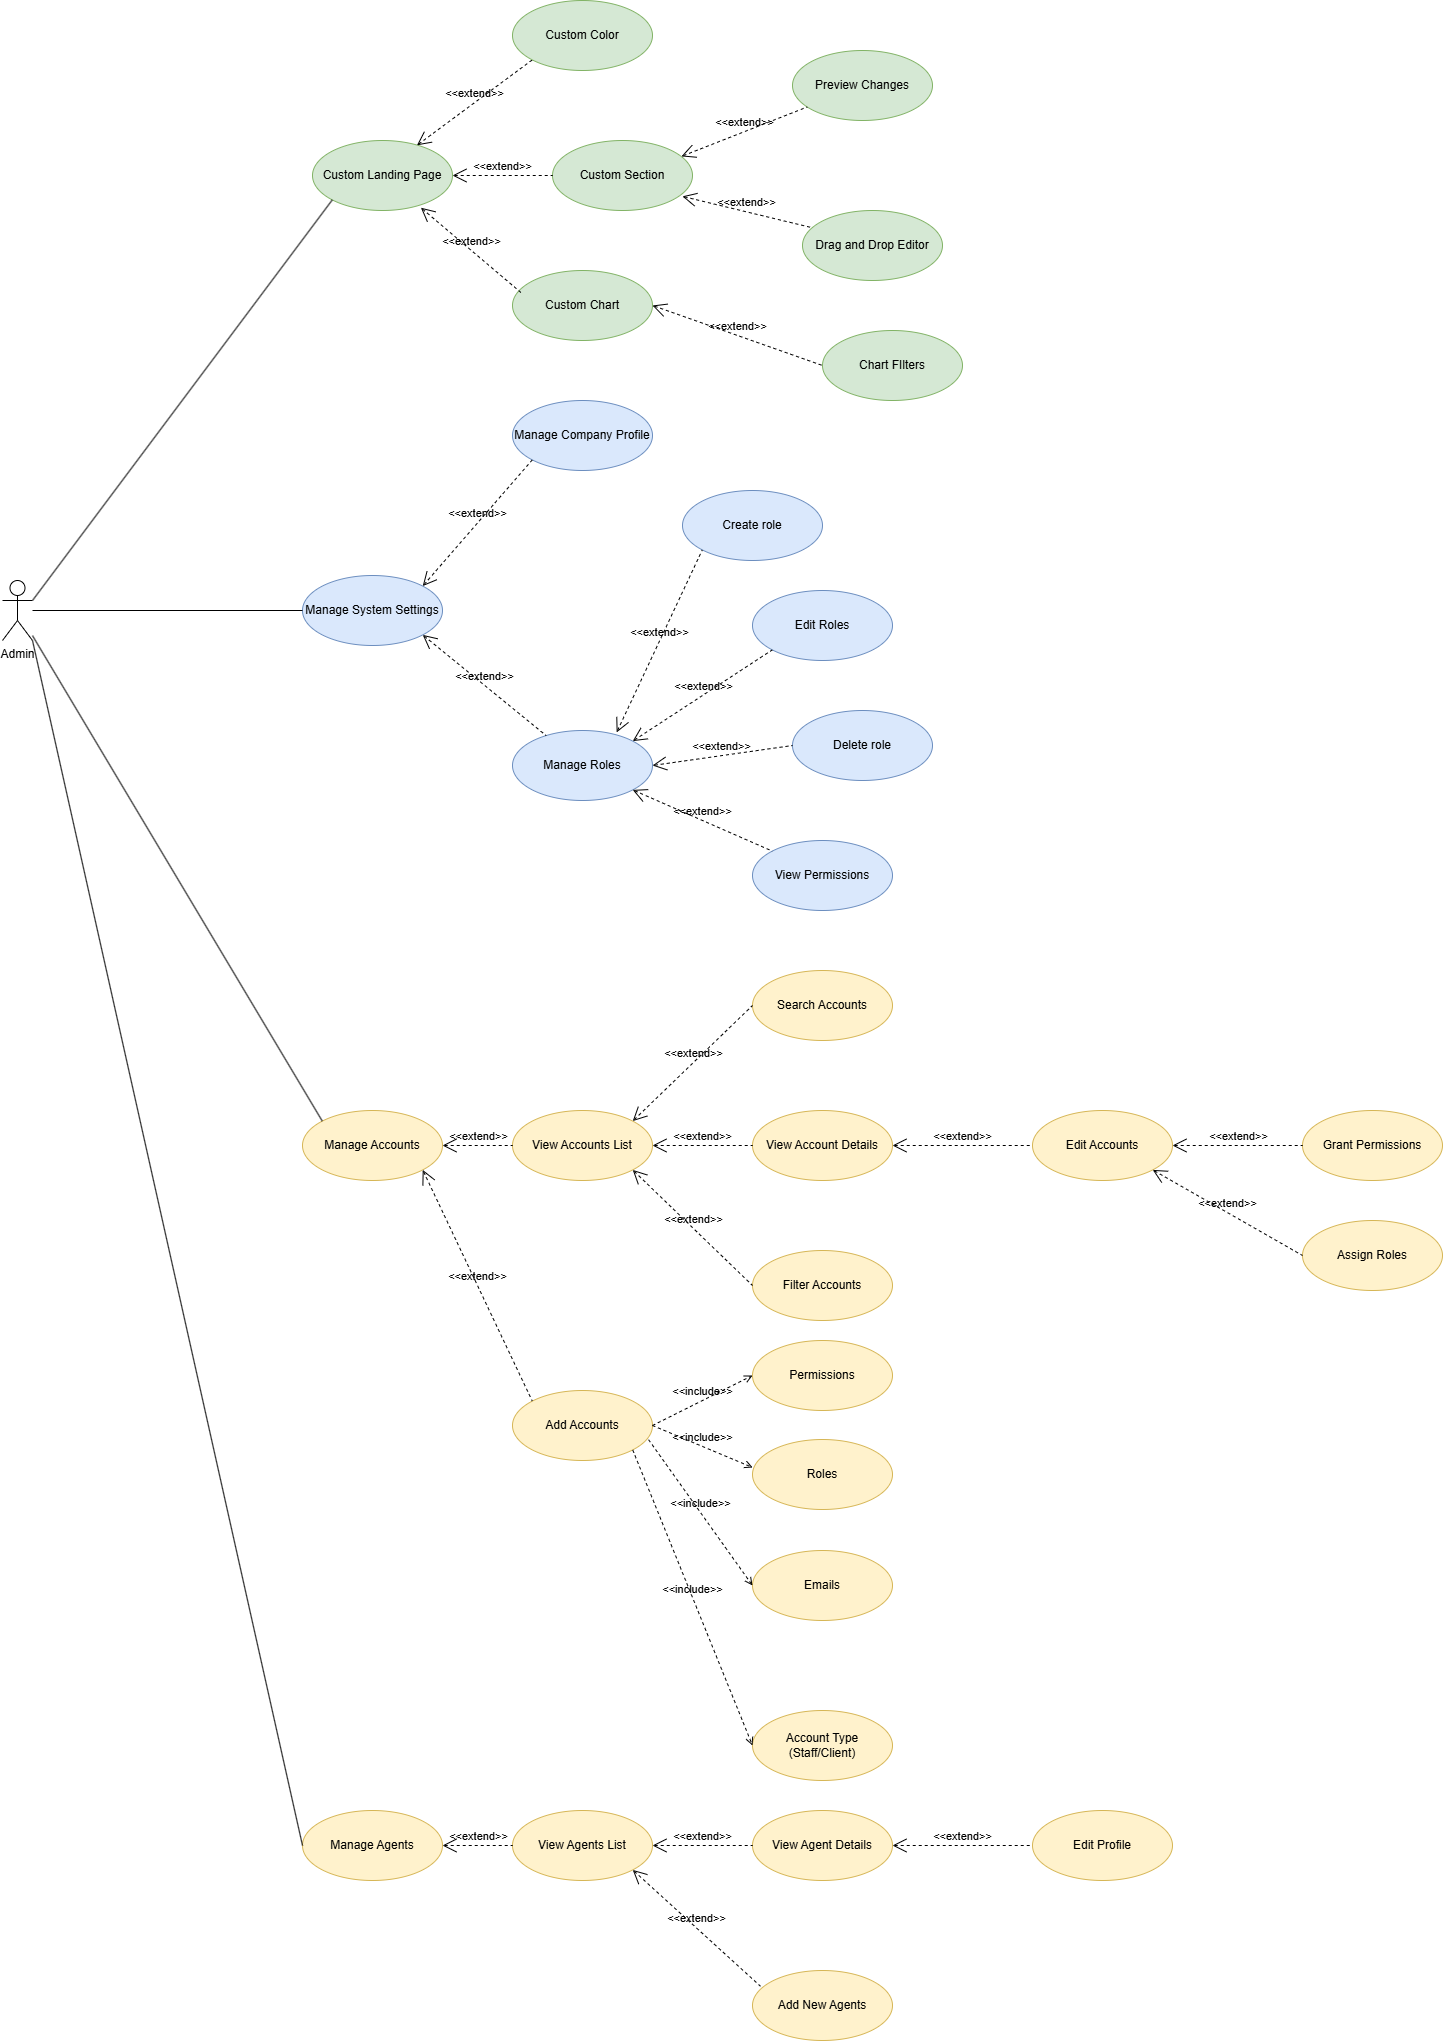
\includegraphics[width=10cm]{graphics/usecase/freight-flex-UC-Admin.png}
    \caption{Usecase Diagram for Admin}
    \label{fig:Usecase Diagram for Admin}
\end{figure}

\subsubsection{Client Settings}
\begin{table}[H]
\begin{tabularx}{\textwidth}{|p{0.25\textwidth}|X|}
\hline
Usecase name     & Create client                          \\ \hline
Actor            & Admin                                \\ \hline
Description      & Add client            \\ \hline
Preconditions    & Authorized with Super Admin Account. \\ \hline
Postconditions   & Show client details.                   \\ \hline
Normal Flow &
  \begin{tabular}[c]{@{}l@{}}1. Actor go to Clients.\\ 2. Actor click on new client button.\\ 3. Actor fill client information.\\ 4. Actor click on save button.\end{tabular} \\ \hline
Exception Flow &
  \begin{tabular}[c]{@{}l@{}}4a. Email has been used.\\ Cannot create client.\end{tabular} \\ \hline
Alternative Flow &                                      \\ \hline
\end{tabularx}
\caption{Create client}
\label{tab:create-client}
\end{table}

\begin{table}[H]
\begin{tabularx}{\textwidth}{|p{0.25\textwidth}|X|}
\hline
Usecase name     & Update client details                         \\ \hline
Actor            & Admin                                \\ \hline
Description      & Add client            \\ \hline
Preconditions    & Authorized with Super Admin Account. \\ \hline
Postconditions   & Show updated client details.                   \\ \hline
Normal Flow &
  \begin{tabular}[c]{@{}l@{}}1. Actor go to Clients.\\ 2. Actor click on existing client.\\ 3. Actor choose view icon.\\ 4. Actor update client information.\\ 5. Actor click on save button.\end{tabular} \\ \hline
Exception Flow &
  \begin{tabular}[c]{@{}l@{}}4a. Email has been used.\\ Cannot update client.\end{tabular} \\ \hline
Alternative Flow &                                      \\ \hline
\end{tabularx}
\caption{Update client}
\label{tab:update-client}
\end{table}

\subsubsection{Staff Settings}
\begin{table}[H]
\begin{tabularx}{\textwidth}{|p{0.25\textwidth}|X|}
\hline
Usecase name     & Add staff account                           \\ \hline
Actor            & Admin                                       \\ \hline
Description      & Add staff account                           \\ \hline
Preconditions    & Authorized with an Admin Privilege account. \\ \hline
Postconditions   & Add account successful                      \\ \hline
Normal Flow &
  \begin{tabular}[c]{@{}l@{}}1. Actor go to Adminstrantions.\\ 2. Actor choose tab Staff.\\ 3. Actor choose create button.\\ 4. Actor fills required fields.\\ 5. Actor click on save button.\end{tabular} \\ \hline
Exception Flow &
  \begin{tabular}[c]{@{}l@{}}4a. Actor does not fill required fields.\\ 4b. Email has been used.\\ Cannot save staff.\end{tabular} \\ \hline
Alternative Flow &                                             \\ \hline
\end{tabularx}
\caption{Add new staff}
\label{tab:add-staff}
\end{table}

\subsubsection{Privilege Settings}
\begin{table}[H]
\begin{tabularx}{\textwidth}{|p{0.25\textwidth}|X|}
\hline
Usecase name     & Create role                          \\ \hline
Actor            & Admin                                \\ \hline
Description      & Add role            \\ \hline
Preconditions    & Authorized with Super Admin Account. \\ \hline
Postconditions   & Show role details.                   \\ \hline
Normal Flow &
  \begin{tabular}[c]{@{}l@{}}1. Actor go to Settings.\\ 2. Actor choose tab Role.\\ 3. Actor choose add new button.\\ 4. Actor choose type user.\\ 5. Actor add users to the role.\\ 6. Actor click on save button.\end{tabular} \\ \hline
Exception Flow   &                                      \\ \hline
Alternative Flow &
\begin{tabular}[c]{@{}l@{}} 4a. Actor choose type group.\\ 5a. Actor add groups to the role.\\ 6. Actor click on save button.\end{tabular} \\ \hline
\end{tabularx}
\caption{Create new role}
\label{tab:create-role}
\end{table}

\begin{table}[H]
\begin{tabularx}{\textwidth}{|p{0.25\textwidth}|X|}
\hline
Usecase name     & Create permission                          \\ \hline
Actor            & Admin                                \\ \hline
Description      & Add permission            \\ \hline
Preconditions    & Authorized with Super Admin Account. \\ \hline
Postconditions   & Show permission details.                   \\ \hline
Normal Flow &
  \begin{tabular}[c]{@{}l@{}}1. Actor go to Settings.\\ 2. Actor choose tab Permission.\\ 3. Actor choose add new button.\\ 4. Actor fill required fields.\\ 5. Actor add role to the permission.\\ 6. Actor click on save button.\end{tabular} \\ \hline
Exception Flow   &                                      \\ \hline
Alternative Flow &
\begin{tabular}[c]{@{}l@{}}  5a. Actor add groups to the permission.\\ 6. Actor click on save button.\end{tabular} \\ \hline
\end{tabularx}
\caption{Create new permission}
\label{tab:create-permission}
\end{table}

\begin{table}[H]
\begin{tabularx}{\textwidth}{|p{0.25\textwidth}|X|}
\hline
Usecase name     & Create new group                          \\ \hline
Actor            & Admin                                \\ \hline
Description      & Add new group            \\ \hline
Preconditions    & Authorized with Super Admin Account. \\ \hline
Postconditions   & Show group details.                   \\ \hline
Normal Flow &
  \begin{tabular}[c]{@{}l@{}}1. Actor go to Settings.\\ 2. Actor choose tab Group Management.\\ 3. Actor choose add new button.\\ 4. Actor fill required fields.\\ 5. Actor click on save button.\end{tabular} \\ \hline
Exception Flow   &                                      \\ \hline
Alternative Flow &                               \\ \hline
\end{tabularx}
\caption{Create new group}
\label{tab:create-group}
\end{table}

\begin{table}[H]
\begin{tabularx}{\textwidth}{|p{0.25\textwidth}|X|}
\hline
Usecase name     & Update group members                         \\ \hline
Actor            & Admin                                \\ \hline
Description      & Update group members            \\ \hline
Preconditions    & Authorized with Super Admin Account. \\ \hline
Postconditions   & Show group details.                   \\ \hline
Normal Flow &
  \begin{tabular}[c]{@{}l@{}}1. Actor go to Settings.\\ 2. Actor choose tab Group Management.\\ 3. Actor choose existing group.\\ 4. Actor choose add members button.\\ 5. Actor choose memebers to add.\\ 6. Actor click on save button.\end{tabular} \\ \hline
Exception Flow   &                                      \\ \hline
Alternative Flow &
  \begin{tabular}[c]{@{}l@{}}4a. Actor choose existing members.\\  5a. Actor click remove members button.\\ 6. Actor click on save button.\end{tabular} \\ \hline
\end{tabularx}
\caption{Update group members}
\label{tab:update-group-members}
\end{table}

\subsubsection{Provider Settings}
\begin{table}[H]
\begin{tabularx}{\textwidth}{|p{0.25\textwidth}|X|}
\hline
Usecase name     & View provider details                       \\ \hline
Actor            & Admin, Staff                             \\ \hline
Description      & View provider details                       \\ \hline
Preconditions    & Staff has view permission or Admin       \\ \hline
Postconditions   & Display a detailed provider \\ \hline
Normal Flow & \begin{tabular}[c]{@{}l@{}}1. Actor go to Providers.\\ 2. Actor choose action button of Provider to view.\end{tabular} \\ \hline
Exception Flow   & Actor does not have permission to view provider\\ \hline
Alternative Flow &                                          \\ \hline
\end{tabularx}
\caption{View provider details}
\label{tab:provider-detail}
\end{table}

\begin{table}[H]
\begin{tabularx}{\textwidth}{|p{0.25\textwidth}|X|}
\hline
Usecase name     & Search provider                       \\ \hline
Actor            & Admin, Staff                       \\ \hline
Description      & Search provider                       \\ \hline
Preconditions    & Staff has view permission or Admin \\ \hline
Postconditions &
  Display a paginated list of providers related to the search information. \\ \hline
Normal Flow &
  \begin{tabular}[c]{@{}l@{}}1. Actor go to Providers.\\ 2. Actor enter code or name to search.\end{tabular} \\ \hline
Exception Flow   & Keyword search does not match \\ \hline
Alternative Flow &                                    \\ \hline
\end{tabularx}
\caption{Search provider}
\label{tab:provider-search}
\end{table}

\subsection{Usecase Diagram for Staff}
\begin{figure}[H]
    \centering
    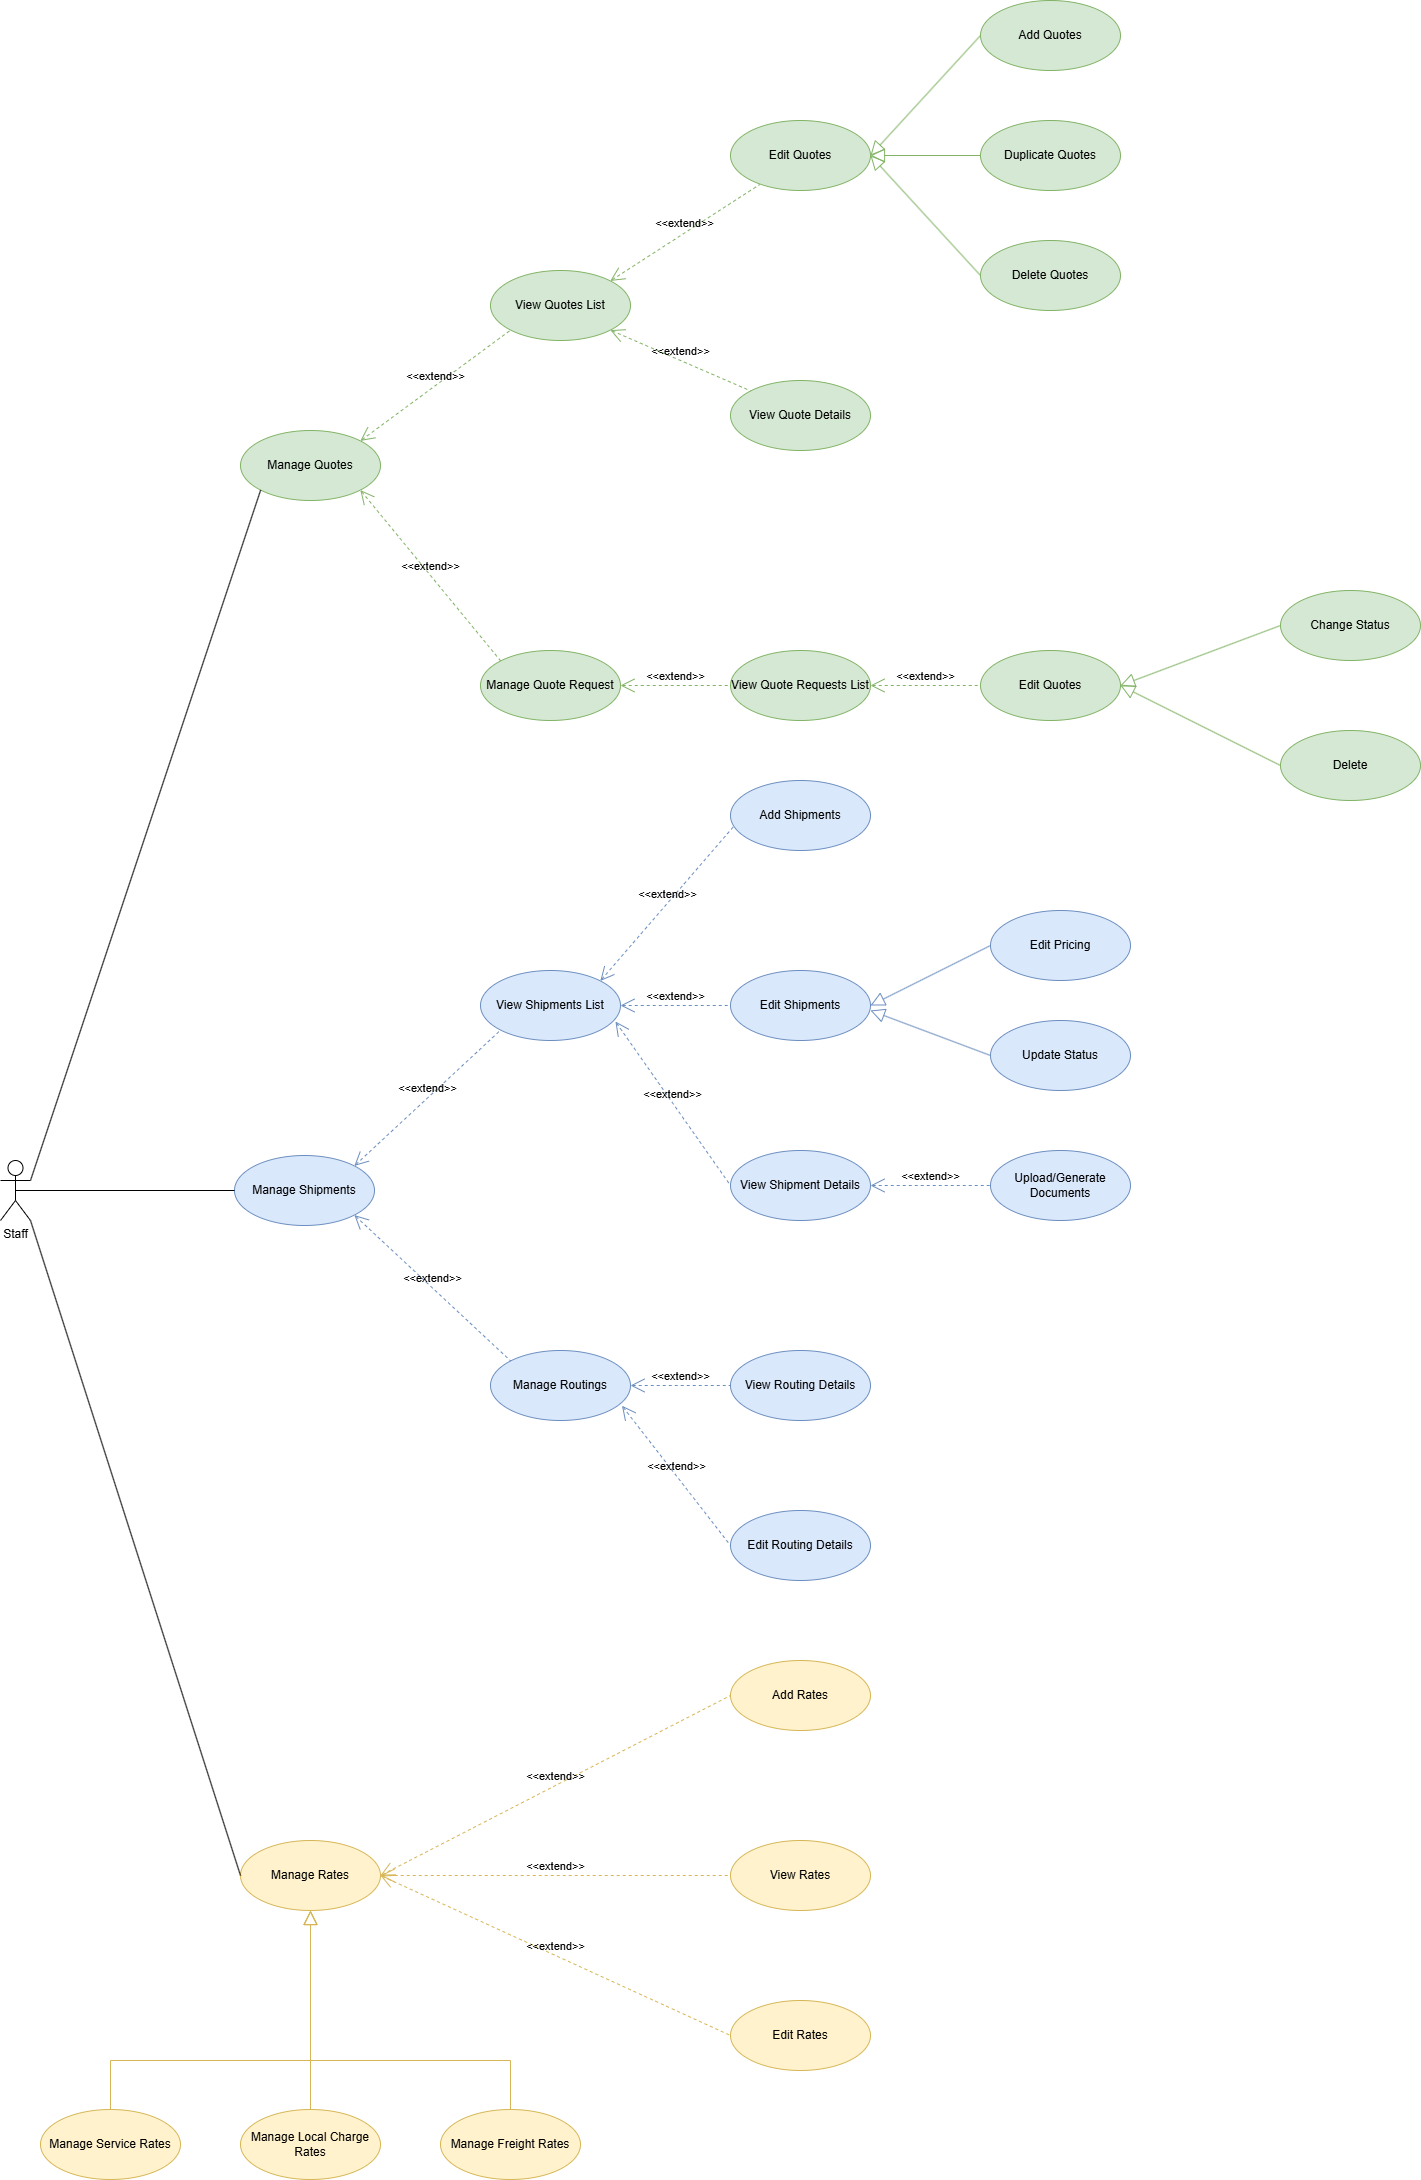
\includegraphics[width=10cm]{graphics/usecase/freight-flex-UC-Staff.png}
    \caption{Usecase Diagram for Staff}
    \label{fig:Usecase Diagram for Staff}
\end{figure}

\subsubsection{Rate Settings}
\begin{table}[H]
\begin{tabularx}{\textwidth}{|p{0.25\textwidth}|X|}
\hline
Usecase name     & Create FCL rate    \\ \hline
Actor            & Staff                           \\ \hline
Description      & Add FCL rate    \\ \hline
Preconditions    & Staff has create rate permission \\ \hline
Postconditions   & Create rate successful                  \\ \hline
Normal Flow &
  \begin{tabular}[c]{@{}l@{}}1. Actor go to Rates\\ 2. Actor choose tab Road FCL.\\ 3. Actor choose add new button.\\ 4. Actor fill required fields.\\ 5. Actor click on save button.\end{tabular} \\ \hline
Exception Flow   &                                         \\ \hline
Alternative Flow &                                         \\ \hline
\end{tabularx}
\caption{Create FCL rate}
\label{tab:create-fcl-rate}
\end{table}

\begin{table}[H]
\begin{tabularx}{\textwidth}{|p{0.25\textwidth}|X|}
\hline
Usecase name     & Create charge type    \\ \hline
Actor            & Staff                           \\ \hline
Description      & Add charge type    \\ \hline
Preconditions    & Staff has create rate permission \\ \hline
Postconditions   & Create charge type successful                  \\ \hline
Normal Flow &
  \begin{tabular}[c]{@{}l@{}}1. Actor go to Settings\\ 2. Actor choose tab Charge Type Management.\\ 3. Actor choose add new button.\\ 4. Actor fill required fields.\\ 5. Actor click on save button.\end{tabular} \\ \hline
Exception Flow   &                                         \\ \hline
Alternative Flow &                                         \\ \hline
\end{tabularx}
\caption{Create charge type}
\label{tab:create-charge-type}
\end{table}

\begin{table}[H]
  \begin{tabularx}{\textwidth}{|p{0.25\textwidth}|X|}
  \hline
  Usecase name     & Create service charge    \\ \hline
  Actor            & Staff                           \\ \hline
  Description      & Add service charge    \\ \hline
  Preconditions    & Staff has create rate permission \\ \hline
  Postconditions   & Create service charge successful                  \\ \hline
  Normal Flow &
    \begin{tabular}[c]{@{}l@{}}1. Actor go to Rates\\ 2. Actor choose tab Service Charge.\\ 3. Actor choose add new button.\\ 4. Actor fill required fields.\\ 5. Actor click on save button.\end{tabular} \\ \hline
  Exception Flow   & 
    \begin{tabular}[c]{@{}l@{}}4a.There is not charge type available.\\ Cannot create service charge.\end{tabular}\\ \hline
  Alternative Flow &                                         \\ \hline
  \end{tabularx}
  \caption{Create service charge}
  \label{tab:create-service-charge}
  \end{table}

\subsubsection{Quote Settings}
\begin{table}[H]
\begin{tabularx}{\textwidth}{|p{0.25\textwidth}|X|}
\hline
Usecase name     & View Quote Request list                    \\ \hline
Actor            & Staff                                      \\ \hline
Description      & View all quote requests.                   \\ \hline
Preconditions    & Staff has view quote permission            \\ \hline
Postconditions   & Display a paginated list of quote requests \\ \hline
Normal Flow & \begin{tabular}[c]{@{}l@{}}1. Actor go to Quotes.\\ 2. Actor go to Quote Request tab.\end{tabular} \\ \hline
Exception Flow   &                                            \\ \hline
Alternative Flow &                                            \\ \hline
\end{tabularx}
\caption{View Quote Request list}
\label{tab:quote-request-list}
\end{table}

\begin{table}[H]
\begin{tabularx}{\textwidth}{|p{0.25\textwidth}|X|}
\hline
Usecase name     & View Quote Request detail       \\ \hline
Actor            & Staff                           \\ \hline
Description      & View quote request detail.      \\ \hline
Preconditions    & Staff has view quote permission \\ \hline
Postconditions   & Display quote request detail    \\ \hline
Normal Flow & \begin{tabular}[c]{@{}l@{}}1. Actor go to Quotations.\\ 2. Actor go to Quote Request tab.\\ 3. Actor choose a quote request.\end{tabular} \\ \hline
Exception Flow   &                                 \\ \hline
Alternative Flow &                                 \\ \hline
\end{tabularx}
\caption{View Quote Request detail}
\label{tab:quote-request-detail}
\end{table}

\begin{table}[H]
\begin{tabularx}{\textwidth}{|p{0.25\textwidth}|X|}
\hline
Usecase name     & Create quote from request                        \\ \hline
Actor            & Staff                                            \\ \hline
Description      & Generate a quote from the quote request          \\ \hline
Preconditions    & Staff has view, create and edit quote permission \\ \hline
Postconditions   & Create quote successful                          \\ \hline
Normal Flow &
  \begin{tabular}[c]{@{}l@{}}1. Actor go to Quotations.\\ 2. Actor go to Quote Request tab.\\ 3. Actor choose a quote request.\\ 4. Actor choose create quote from request button.\\ 5. Actor fill required fields.\\ 6. Actor click on save button.\end{tabular} \\ \hline
Exception Flow   &                                                  \\ \hline
Alternative Flow &                                                  \\ \hline
\end{tabularx}
\caption{Create quote from request}
\label{tab:quote-create-from-request}
\end{table}

\begin{table}[H]
\begin{tabularx}{\textwidth}{|p{0.25\textwidth}|X|}
\hline
Usecase name     & Create quote                        \\ \hline
Actor            & Staff                                            \\ \hline
Description      & Generate a quote         \\ \hline
Preconditions    & Staff has view, create and edit quote permission \\ \hline
Postconditions   & Create quote successful                          \\ \hline
Normal Flow &
  \begin{tabular}[c]{@{}l@{}}1. Actor go to Quotations.\\ 2. Actor go to Quote tab.\\ 3. Actor choose create new button.\\4. Actor fill required fields.\\ 5. Actor click on save button.\end{tabular} \\ \hline
Exception Flow   &                                                  \\ \hline
Alternative Flow &                                                  \\ \hline
\end{tabularx}
\caption{Create quote}
\label{tab:quote-create}
\end{table}

\begin{table}[H]
\begin{tabularx}{\textwidth}{|p{0.25\textwidth}|X|}
\hline
Usecase name     & Search quotes                       \\ \hline
Actor            & Admin, Staff                       \\ \hline
Description      & Search quotes                       \\ \hline
Preconditions    & Staff has view quote permission or Admin \\ \hline
Postconditions &
  Display a paginated list of quotes related to the search information. \\ \hline
Normal Flow &
  \begin{tabular}[c]{@{}l@{}}1. Actor go to Quotations.\\ 2. Actor go to Quote tab.\\3. Actor enter code to search.\end{tabular} \\ \hline
Exception Flow   & Keyword search does not match \\ \hline
Alternative Flow &                                    \\ \hline
\end{tabularx}
\caption{Search quotes}
\label{tab:quote-search}
\end{table}

\begin{table}[H]
\begin{tabularx}{\textwidth}{|p{0.25\textwidth}|X|}
\hline
Usecase name     & Search quotes filter field                     \\ \hline
Actor            & Admin, Staff                       \\ \hline
Description      & Search quote filter specific field                      \\ \hline
Preconditions    & Staff has view quote permission or Admin \\ \hline
Postconditions &
  Display a paginated list of quotes related to the search information. \\ \hline
Normal Flow &
  \begin{tabular}[c]{@{}l@{}}1. Actor go to Quotations.\\ 2. Actor go to Quote tab.\\3. Actor click on search filter button.\\4. Actor choose field to search.\\5. Actor click on apply button.\end{tabular} \\ \hline
Exception Flow   & Keyword search does not match \\ \hline
Alternative Flow &                                    \\ \hline
\end{tabularx}
\caption{Search quotes filter field}
\label{tab:quote-search-filter-field}
\end{table}

\begin{table}[H]
\begin{tabularx}{\textwidth}{|p{0.25\textwidth}|X|}
\hline
Usecase name     & Sort quotes                       \\ \hline
Actor            & Admin, Staff                       \\ \hline
Description      & Sort quotes                       \\ \hline
Preconditions    & Staff has view quote permission or Admin \\ \hline
Postconditions &
  Display a paginated list of quotes related to the sorted column. \\ \hline
Normal Flow &
  \begin{tabular}[c]{@{}l@{}}1. Actor go to Quotations.\\ 2. Actor go to Quote tab.\\3. Actor choose column to sort.\end{tabular} \\ \hline
Exception Flow   &  \\ \hline
Alternative Flow &                                    \\ \hline
\end{tabularx}
\caption{Sort quotes}
\label{tab:quote-sort}
\end{table}

\subsubsection{Shipment Settings}
\begin{table}[H]
\begin{tabularx}{\textwidth}{|p{0.25\textwidth}|X|}
\hline
Usecase name     & Add shipment               \\ \hline
Actor            & Staff                      \\ \hline
Description      & Add a shipment             \\ \hline
Preconditions &
  \begin{tabular}[c]{@{}l@{}}1. Staff has create shipment permission.\\ 2. A quote is created.\end{tabular} \\ \hline
Postconditions   & Create shipment successful \\ \hline
Normal Flow &
  \begin{tabular}[c]{@{}l@{}}1. Actor go to Quotations.\\ 2. Actor go to Quote tab.\\ 3. Actor choose a quote not booked.\\ 4. Actor choose create shipment button.\\ 5. Actor update shipment information.\\ 6. Actor click on save button.\end{tabular} \\ \hline
Exception Flow   &                            \\ \hline
Alternative Flow &                            \\ \hline
\end{tabularx}
\caption{Create shipment from quote}
\label{tab:shipment-create-from-quote}
\end{table}

\begin{table}[H]
\begin{tabularx}{\textwidth}{|p{0.25\textwidth}|X|}
\hline
Usecase name     & View shipment               \\ \hline
Actor            & Staff                      \\ \hline
Description      & View a shipment             \\ \hline
Preconditions & Staff has view shipment permission. \\ \hline
Postconditions   & Display shipment detail. \\ \hline
Normal Flow &
  \begin{tabular}[c]{@{}l@{}}1. Actor go to Shipments.\\ 2. Actor choose a shipment.\\ 3. Actor click on view shipment button.\end{tabular} \\ \hline
Exception Flow   &                            \\ \hline
Alternative Flow &                            \\ \hline
\end{tabularx}
\caption{View shipment}
\label{tab:shipment-view}
\end{table}

\begin{table}[H]
\begin{tabularx}{\textwidth}{|p{0.25\textwidth}|X|}
\hline
Usecase name     & Upload shipment document               \\ \hline
Actor            & Staff                      \\ \hline
Description      & Upload related documents to shipment             \\ \hline
Preconditions & Staff has shipment permission. \\ \hline
Postconditions   & Display shipment detail. \\ \hline
Normal Flow &
  \begin{tabular}[c]{@{}l@{}}1. Actor go to Shipments.\\ 2. Actor choose a shipment.\\ 3. Actor click on view shipment button.\\ 4. Actor click Document tab.\\ 5. Actor upload new document.\\ 6. Actor click on save button.\\\end{tabular} \\ \hline
Exception Flow   &                            \\ \hline
Alternative Flow &                            \\ \hline
\end{tabularx}
\caption{Upload shipment document}
\label{tab:shipment-upload-document}
\end{table}

\begin{table}[H]
\begin{tabularx}{\textwidth}{|p{0.25\textwidth}|X|}
\hline
Usecase name     & Add shipment debit note               \\ \hline
Actor            & Staff                      \\ \hline
Description      & Add credit/debit note to shipment             \\ \hline
Preconditions & Staff has shipment permission. \\ \hline
Postconditions   & Add credit/debit note successful. \\ \hline
Normal Flow &
  \begin{tabular}[c]{@{}l@{}}1. Actor go to Shipments.\\ 2. Actor choose a shipment.\\ 3. Actor click on view shipment button.\\ 4. Actor click Profit and Loss tab.\\ 5. Actor add new credit/debit note.\\ 6. Actor click on save button.\\\end{tabular} \\ \hline
Exception Flow   &                            \\ \hline
Alternative Flow &                            \\ \hline
\end{tabularx}
\caption{Add shipment debit note}
\label{tab:shipment-debit-not}
\end{table}

\begin{table}[H]
\begin{tabularx}{\textwidth}{|p{0.25\textwidth}|X|}
\hline
Usecase name     & View shipment profit and loss               \\ \hline
Actor            & Staff                      \\ \hline
Description      & View a shipment             \\ \hline
Preconditions & Staff has view shipment permission. \\ \hline
Postconditions   & Display shipment profit and loss. \\ \hline
Normal Flow &
  \begin{tabular}[c]{@{}l@{}}1. Actor go to Shipments.\\ 2. Actor choose a shipment.\\ 3. Actor click on view shipment button.\\ 4. Actor click Profit and Loss tab.\end{tabular} \\ \hline
Exception Flow   &                            \\ \hline
Alternative Flow &                            \\ \hline
\end{tabularx}
\caption{View shipment profit and loss}
\label{tab:shipment-profit-view}
\end{table}

\subsection{Usecase Diagram for Client}
\begin{figure}[H]
    \centering
    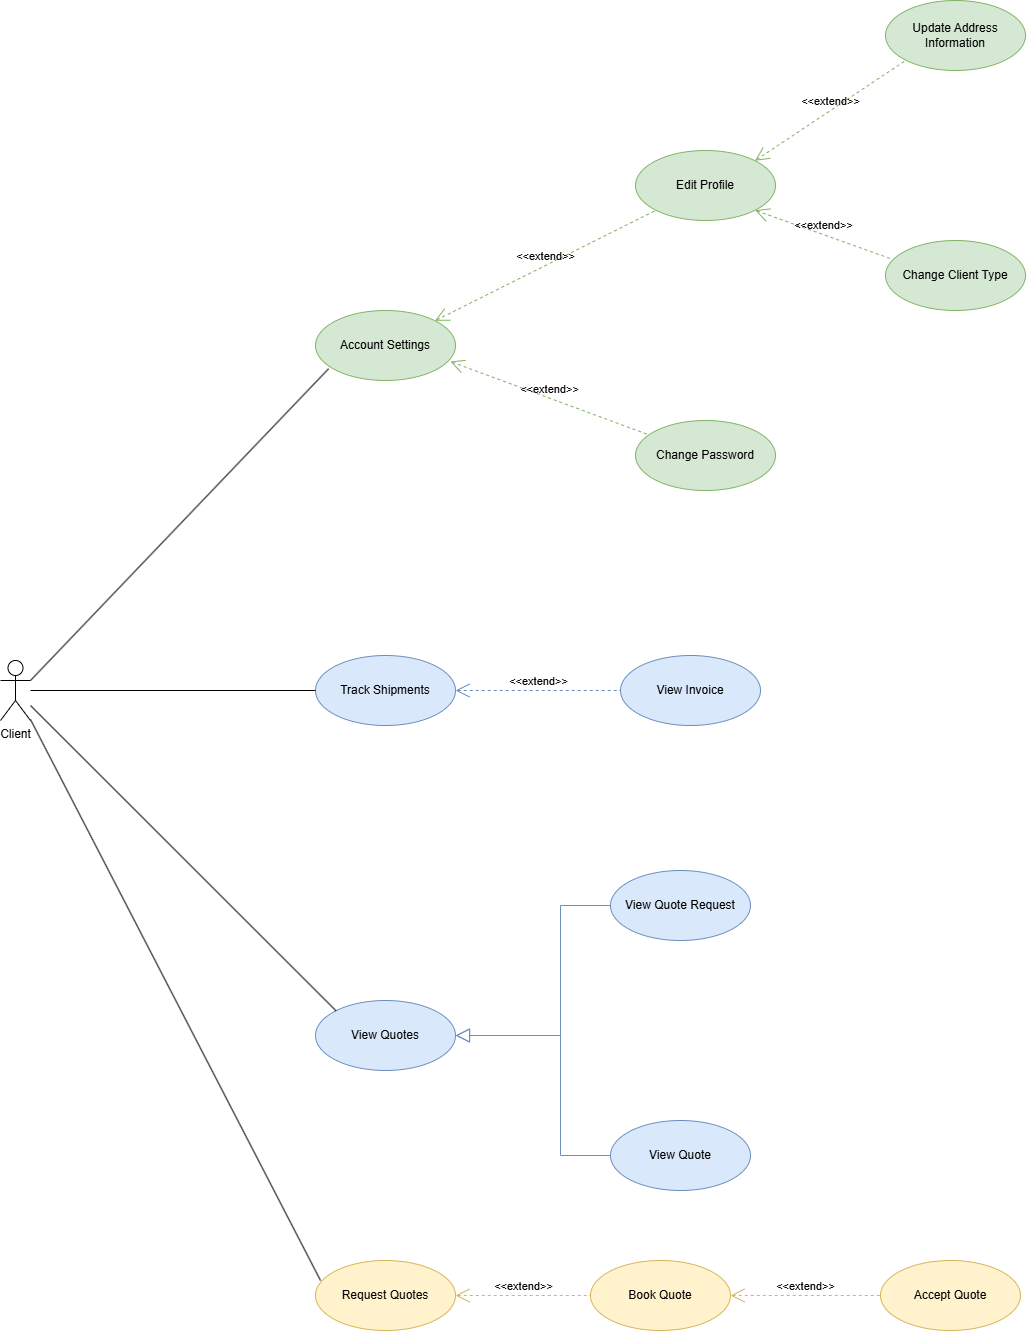
\includegraphics[width=10cm]{graphics/usecase/freight-flex-UC-Client.png}
    \caption{Usecase Diagram for Client}
    \label{fig:Usecase Diagram for Client}
\end{figure}

\subsubsection{Quote Settings}
\begin{table}[H]
\begin{tabularx}{\textwidth}{|p{0.25\textwidth}|X|}
\hline
Usecase name     & Create quote request                  \\ \hline
Actor            & Client                                 \\ \hline
Description      & Create quote request                     \\ \hline
Preconditions    & 1. Client has create quote request permission. \\ \hline
Postconditions   & Display quote request detail         \\ \hline
Normal Flow & \begin{tabular}[c]{@{}l@{}}1. Actor go to Quotes.\\ 2. Actor choose tab quote request.\\ 3. Actor click on add new button.\\4. Actor fill required fields.\\ 5. Actor click on save button. \end{tabular} \\ \hline
Exception Flow   &                                        \\ \hline
Alternative Flow &                                        \\ \hline
\end{tabularx}
\caption{Create quote request}
\label{tab:quote-request-create}
\end{table}

\begin{table}[H]
  \begin{tabularx}{\textwidth}{|p{0.25\textwidth}|X|}
  \hline
  Usecase name     & Create quote request from landing page                 \\ \hline
  Actor            & Client                                 \\ \hline
  Description      & Create quote request from landing page                    \\ \hline
  Preconditions    &   \\ \hline
  Postconditions   & Create and send to staff         \\ \hline
  Normal Flow & \begin{tabular}[c]{@{}l@{}}1. Actor go to Landing Page.\\ 2. Actor choose Quote request.\\3. Actor fill required fields.\\ 4. Actor click on send button. \end{tabular} \\ \hline
  Exception Flow   &                                        \\ \hline
  Alternative Flow &                                        \\ \hline
  \end{tabularx}
  \caption{Create quote requestfrom landing page}
  \label{tab:quote-request-create-landing-page}
  \end{table}

\begin{table}[H]
\begin{tabularx}{\textwidth}{|p{0.25\textwidth}|X|}
\hline
Usecase name     & Send quote request to staff                  \\ \hline
Actor            & Client                                 \\ \hline
Description      & Send quote request to staff                     \\ \hline
Preconditions    & 1. Client has create quote request permission. \\ \hline
Postconditions   & Send to staff successful         \\ \hline
Normal Flow & \begin{tabular}[c]{@{}l@{}}1. Actor go to Quotes.\\ 2. Actor choose tab quote request.\\ 3. Actor click on existing quote request.\\ 4. Actor click on send button. \end{tabular} \\ \hline
Exception Flow   &                                        \\ \hline
Alternative Flow &                                        \\ \hline
\end{tabularx}
\caption{Send quote request}
\label{tab:quote-request-send}
\end{table}

\subsubsection{Shipment Settings}
\begin{table}[H]
\begin{tabularx}{\textwidth}{|p{0.25\textwidth}|X|}
\hline
Usecase name     & View shipment status                   \\ \hline
Actor            & Client                                 \\ \hline
Description      & View shipment status                   \\ \hline
Preconditions    & 1. Clien has view shipment permission. \\ \hline
Postconditions   & Display shipment status detail         \\ \hline
Normal Flow & \begin{tabular}[c]{@{}l@{}}1. Actor go to Shipments.\\ 2. Actor choose a shipment.\end{tabular} \\ \hline
Exception Flow   &                                        \\ \hline
Alternative Flow &                                        \\ \hline
\end{tabularx}
\caption{View shipment status}
\label{tab:shipment-status-view}
\end{table}

\begin{table}[H]
\begin{tabularx}{\textwidth}{|p{0.25\textwidth}|X|}
\hline
Usecase name     & Seach shipment                                                          \\ \hline
Actor            & Client                                                                  \\ \hline
Description      & View a paginated list of shipments related to the search information    \\ \hline
Preconditions    & 1. Clien has view shipment permission.                                  \\ \hline
Postconditions   & Display a paginated list of shipments related to the search information \\ \hline
Normal Flow &
  \begin{tabular}[c]{@{}l@{}}1. Actor go to Shipments.\\ 2. Actor clicks to Search.\\ 3. Actor enters information to search.\\ 4. Actor clicks search button\end{tabular} \\ \hline
Exception Flow   & Search keyword does not match any shipments                             \\ \hline
Alternative Flow &                                                                         \\ \hline
\end{tabularx}
\caption{Seach shipment}
\label{tab:shipment-search}
\end{table}